%File: formatting-instructions-latex-2025.tex
%release 2025.0
\documentclass[letterpaper]{article} % DO NOT CHANGE THIS
\usepackage{aaai25}  % DO NOT CHANGE THIS
\usepackage{times}  % DO NOT CHANGE THIS
\usepackage{helvet}  % DO NOT CHANGE THIS
\usepackage{courier}  % DO NOT CHANGE THIS
\usepackage[hyphens]{url}  % DO NOT CHANGE THIS
\usepackage{graphicx} % DO NOT CHANGE THIS
\urlstyle{rm} % DO NOT CHANGE THIS
\def\UrlFont{\rm}  % DO NOT CHANGE THIS
\usepackage{natbib}  % DO NOT CHANGE THIS AND DO NOT ADD ANY OPTIONS TO IT
\usepackage{caption} % DO NOT CHANGE THIS AND DO NOT ADD ANY OPTIONS TO IT
\frenchspacing  % DO NOT CHANGE THIS
\setlength{\pdfpagewidth}{8.5in}  % DO NOT CHANGE THIS
\setlength{\pdfpageheight}{11in}  % DO NOT CHANGE THIS
%
% These are recommended to typeset algorithms but not required. See the subsubsection on algorithms. Remove them if you don't have algorithms in your paper.
\usepackage{algorithm}
\usepackage{algorithmic}
\usepackage{amsmath}
\usepackage{tabularx}
\usepackage{makecell}
\usepackage{multirow}
\usepackage{multicol}
%\usepackage{balance}
\usepackage{booktabs}

%
% These are are recommended to typeset listings but not required. See the subsubsection on listing. Remove this block if you don't have listings in your paper.
\usepackage{newfloat}
\usepackage{listings}
\DeclareCaptionStyle{ruled}{labelfont=normalfont,labelsep=colon,strut=off} % DO NOT CHANGE THIS
\lstset{%
	basicstyle={\footnotesize\ttfamily},% footnotesize acceptable for monospace
	numbers=left,numberstyle=\footnotesize,xleftmargin=2em,% show line numbers, remove this entire line if you don't want the numbers.
	aboveskip=0pt,belowskip=0pt,%
	showstringspaces=false,tabsize=2,breaklines=true}
\floatstyle{ruled}
\newfloat{listing}{tb}{lst}{}
\floatname{listing}{Listing}
%
% Keep the \pdfinfo as shown here. There's no need
% for you to add the /Title and /Author tags.
\pdfinfo{
/TemplateVersion (2025.1)
}

% DISALLOWED PACKAGES
% \usepackage{authblk} -- This package is specifically forbidden
% \usepackage{balance} -- This package is specifically forbidden
% \usepackage{color (if used in text)
% \usepackage{CJK} -- This package is specifically forbidden
% \usepackage{float} -- This package is specifically forbidden
% \usepackage{flushend} -- This package is specifically forbidden
% \usepackage{fontenc} -- This package is specifically forbidden
% \usepackage{fullpage} -- This package is specifically forbidden
% \usepackage{geometry} -- This package is specifically forbidden
% \usepackage{grffile} -- This package is specifically forbidden
% \usepackage{hyperref} -- This package is specifically forbidden
% \usepackage{navigator} -- This package is specifically forbidden
% (or any other package that embeds links such as navigator or hyperref)
% \indentfirst} -- This package is specifically forbidden
% \layout} -- This package is specifically forbidden
% \multicol} -- This package is specifically forbidden
% \nameref} -- This package is specifically forbidden
% \usepackage{savetrees} -- This package is specifically forbidden
% \usepackage{setspace} -- This package is specifically forbidden
% \usepackage{stfloats} -- This package is specifically forbidden
% \usepackage{tabu} -- This package is specifically forbidden
% \usepackage{titlesec} -- This package is specifically forbidden
% \usepackage{tocbibind} -- This package is specifically forbidden
% \usepackage{ulem} -- This package is specifically forbidden
% \usepackage{wrapfig} -- This package is specifically forbidden
% DISALLOWED COMMANDS
\nocopyright %-- Your paper will not be published if you use this command
% \addtolength -- This command may not be used
% \balance -- This command may not be used
% \baselinestretch -- Your paper will not be published if you use this command
% \clearpage -- No page breaks of any kind may be used for the final version of your paper
% \columnsep -- This command may not be used
% \newpage -- No page breaks of any kind may be used for the final version of your paper
% \pagebreak -- No page breaks of any kind may be used for the final version of your paperr
% \pagestyle -- This command may not be used
% \tiny -- This is not an acceptable font size.
% \vspace{- -- No negative value may be used in proximity of a caption, figure, table, section, subsection, subsubsection, or reference
% \vskip{- -- No negative value may be used to alter spacing above or below a caption, figure, table, section, subsection, subsubsection, or reference

\setcounter{secnumdepth}{0} %May be changed to 1 or 2 if section numbers are desired.

% The file aaai25.sty is the style file for AAAI Press
% proceedings, working notes, and technical reports.
%

% Title

% Your title must be in mixed case, not sentence case.
% That means all verbs (including short verbs like be, is, using,and go),
% nouns, adverbs, adjectives should be capitalized, including both words in hyphenated terms, while
% articles, conjunctions, and prepositions are lower case unless they
% directly follow a colon or long dash
\title{Rethinking Relation Extraction: Beyond Shortcuts to Generalization with a Debiased Benchmark}
\author{
    %Authors
    % All authors must be in the same font size and format.
%    Written by AAAI Press Staff\textsuperscript{\rm 1}\thanks{With help from the AAAI Publications Committee.}\\
%    Francisco Cruz\equalcontrib,
    Liang He, Yougang Chu, Zhen Wu, Jianbing Zhang, Xinyu Dai, Jiajun Chen \\
}
\affiliations{
    %Afiliations
    National Key Laboratory for Novel Software Technology, Nanjing University
%    \textsuperscript{\rm 1}Association for the Advancement of Artificial Intelligence\\
    % If you have multiple authors and multiple affiliations
    % use superscripts in text and roman font to identify them.
    % For example,

    % Sunil Issar\textsuperscript{\rm 2}, 
    % J. Scott Penberthy\textsuperscript{\rm 3}, 
    % George Ferguson\textsuperscript{\rm 4},
    % Hans Guesgen\textsuperscript{\rm 5}
    % Note that the comma should be placed after the superscript

    % email address must be in roman text type, not monospace or sans serif
    heliang@smail.nju.edu.cn
%
% See more examples next
}

%Example, Single Author, ->> remove \iffalse,\fi and place them surrounding AAAI title to use it
\iffalse
\title{My Publication Title --- Single Author}
\author {
    Author Name
}
\affiliations{
    Affiliation\\
    Affiliation Line 2\\
    name@example.com
}
\fi

\iffalse
%Example, Multiple Authors, ->> remove \iffalse,\fi and place them surrounding AAAI title to use it
\title{My Publication Title --- Multiple Authors}
\author {
    % Authors
    First Author Name\textsuperscript{\rm 1,\rm 2},
    Second Author Name\textsuperscript{\rm 2},
    Third Author Name\textsuperscript{\rm 1}
}
\affiliations {
    % Affiliations
    \textsuperscript{\rm 1}Affiliation 1\\
    \textsuperscript{\rm 2}Affiliation 2\\
    firstAuthor@affiliation1.com, secondAuthor@affilation2.com, thirdAuthor@affiliation1.com
}
\fi


% REMOVE THIS: bibentry
% This is only needed to show inline citations in the guidelines document. You should not need it and can safely delete it.
\usepackage{bibentry}
% END REMOVE bibentry

\begin{document}

\maketitle

\begin{abstract}
Benchmarks are crucial for evaluating machine learning algorithm performance, facilitating comparison and identifying superior solutions. However, biases within datasets can lead models to learn shortcut patterns, resulting in inaccurate assessments and hindering real-world applicability. This paper addresses the issue of entity bias in relation extraction tasks, where models tend to rely on entity mentions rather than context. We propose a debiased relation extraction benchmark DREB that breaks the pseudo-correlation between entity mentions and relation types through entity replacement. DREB utilizes Bias Evaluator and PPL Evaluator to ensure low bias and high naturalness, providing a reliable and accurate assessment of model generalization in entity bias scenarios. To establish a new baseline on DREB, we introduce MixDebias, a debiasing method combining data-level and model training-level techniques. MixDebias effectively improves model performance on DREB while maintaining performance on the original dataset. Extensive experiments demonstrate the effectiveness and robustness of MixDebias compared to existing methods, highlighting its potential for improving the generalization ability of relation extraction models. We will release DREB and MixDebias publicly.
\end{abstract}

% Uncomment the following to link to your code, datasets, an extended version or similar.
%
% \begin{links}
%     \link{Code}{https://aaai.org/example/code}
%     \link{Datasets}{https://aaai.org/example/datasets}
%     \link{Extended version}{https://aaai.org/example/extended-version}
% \end{links}

\section{Introduction}

%In the field of machine learning, benchmarks serve as critical tools for evaluating algorithm performance, playing an essential role in comparing different methods and identifying superior solutions using standardized datasets and task setups. However, as model design and evaluation become increasingly reliant on specific datasets, biases within these datasets can lead models to learn shortcut patterns, resulting in inaccurate assessments and hindering their real-world applicability.
%Several studies have shown that improved model performance may not stem from enhanced semantic understanding but rather from learning dataset biases. For instance, in natural language inference tasks, \cite{gururangan2018annotation} discovered a strong correlation between categories and the frequency of negation words on SNLI \cite{bowman2015large} and MNLI \cite{williams2018broad} datasets. \cite{mccoy2019right} observed that fine-tuned language models on the MNLI dataset tend to predict categories based on lexical overlap ratios. In fact verification tasks, \cite{schuster2019towards} pointed out that models often rely on specific phrases or patterns within the claims rather than contextual relationships between the claim and evidence.

Benchmarks are crucial for evaluating machine learning algorithms, providing standardized datasets to compare methods and identify top performers. However, reliance on specific datasets can introduce biases, causing models to learn shortcut patterns instead of true semantic understanding, which hinders their real-world applicability. Studies show that improved performance often stems from exploiting dataset biases rather than enhanced comprehension. For example, in natural language inference, models tend to predict based on lexical overlap ratios or the presence of negation words on SNLI \cite{bowman2015large} and MNLI \cite{williams2018broad} datasets \cite{gururangan2018annotation,mccoy2019right}, and in fact verification tasks, they often rely on specific phrases rather than the contextual relationship between claims and evidence \cite{schuster2019towards}.

\begin{figure}[htbp]
    \centering
    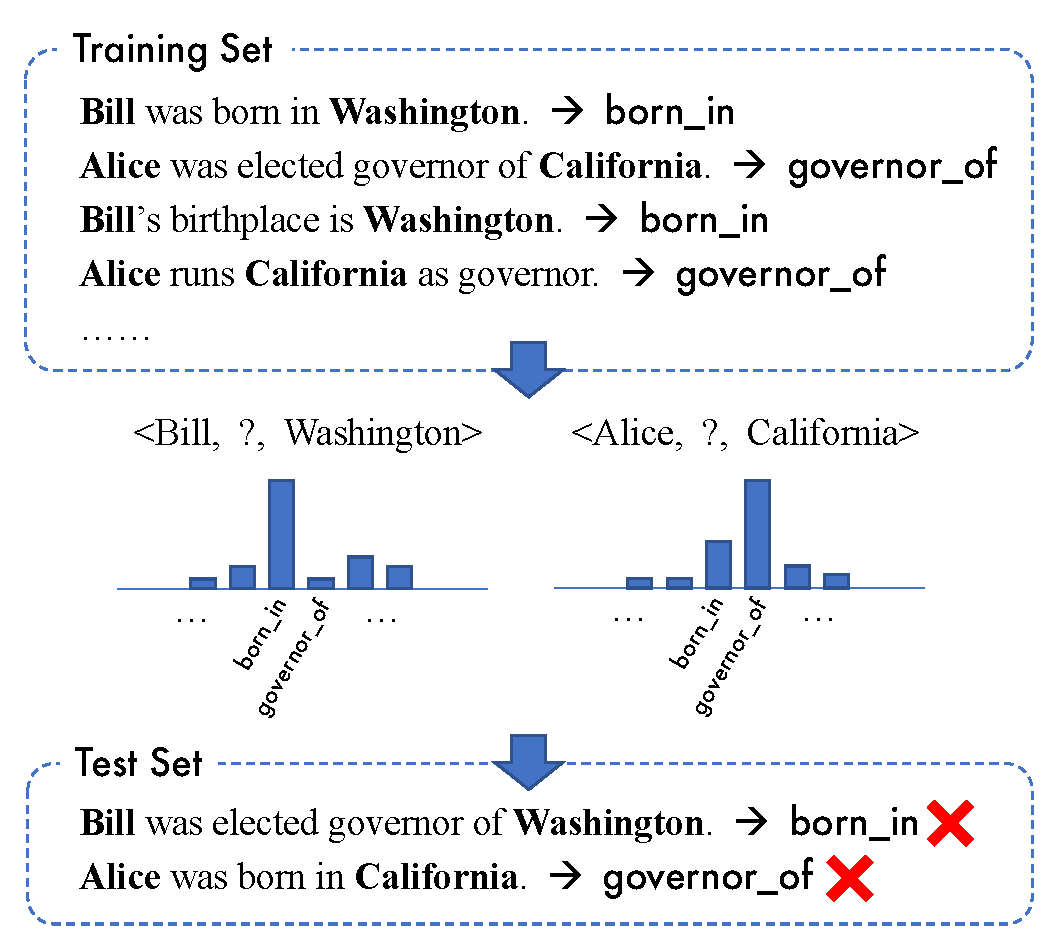
\includegraphics[width=0.4\textwidth]{figure/entity_bias_example.pdf}
    \caption{An illustrative example of how entity biases can cause models to learn false shortcuts, inevitably resulting in erroneous predictions.}
    \label{fig:entity-bias-example}
\end{figure}

%Similar issues exist in relation extraction tasks. A deep analysis of widely used relation extraction datasets such as SemEval 2010 Task 8 \cite{hendrickx2010semeval}, TACRED \cite{zhang2017position}, TACREV \cite{alt2020tacred}, and Re-TACRED \cite{stoica2021re} has found that entity mentions can expose shallow cues for the relation type \cite{zhang2018graph,peng2020learning}. In other words, there is a pseudo-correlation formed between entity mentions and relation types, which is defined as entity bias (Figure \ref{fig:entity-bias-example}). \cite{wang2022should} demonstrated that over half of the instances in the TACRED dataset could be accurately predicted without textual context.
%%He et al. \cite{} confirmed that for some relation types, entity-only inputs yield higher accuracy than context-only inputs. 
%\cite{wang2023fragile} also found that after entity replacement, the performance of state-of-the-art relation extraction models (such as LUKE \cite{yamada2020luke} and IRE \cite{zhou2022improved}) significantly dropped by 30\% - 50\% in terms of F1 scores. \cite{wang2023causal} further discovered that large language models tend to disregard contextual information that contradicts or is infrequently reported in the pre-trained corpus, excessively relying on (biased) parametric knowledge \cite{longpre2021entity} to make unfaithful predictions and perpetuate bias. These prior experiments demonstrate an over-reliance on entities, leading to significant drops in model performance when entity mentions are missing or biased samples are filtered out.

In relation extraction tasks, widely-used datasets like SemEval 2010 Task 8 \cite{hendrickx2010semeval}, TACRED \cite{zhang2017position}, TACREV \cite{alt2020tacred}, and Re-TACRED \cite{stoica2021re} exhibit entity bias, where entity mentions can provide superficial cues for relation types (Figure \ref{fig:entity-bias-example}). This pseudo-correlation between entity mentions and relation types means models can often predict accurately without textual context \cite{zhang2018graph,peng2020learning}. For instance, over half of TACRED instances can be correctly predicted using only entity mentions \cite{wang2022should}. After entity replacement, state-of-the-art models like LUKE \cite{yamada2020luke} and IRE \cite{zhou2022improved} experience significant drops in performance (30\% - 50\% F1 score) \cite{wang2023fragile}. Large language models exacerbate this bias by disregarding contradictory or underrepresented contextual information, overly relying on biased parametric knowledge \cite{longpre2021entity} for predictions \cite{wang2023causal}. These findings highlight a critical over-reliance on entity mentions, severely impacting model performance when entity mentions are absent or debiased.

%Addressing this issue, several approaches have been explored on both the data and model levels. Methods like \cite{wang2022should} and ENTRED \cite{wang2023fragile} aim to reduce biases at the data level, while other research focuses on improving training strategies to enable models to better learn semantic representations. Nonetheless, existing benchmarks still suffer from several shortcomings:
%\begin{itemize}
%    \item At the data level, Existing debiasing dataset construction methods may introduce new biases, affecting evaluation reliability. For example, \cite{wang2022should}'s modification of the TACRED and Re-TACRED datasets resulted in a small number of challenge set samples with a different distribution of relation types compared to the original test set, leading to distribution bias. ENTRED's entity replacement method lacks semantic constraints, potentially introducing semantic bias.
%    \item At the model level, Designing robust debiasing training or prediction strategies to improve model generalization remains an open issue. DFL \cite{mahabadi2020end} modifies the focal loss function to reduce focus on biased samples but may damage in-domain performance and the learning of useful features while reducing bias. R-Drop \cite{liang2021r} utilizes regularization to decrease reliance on specific features but cannot finely control entity biases. CoRE \cite{wang2022should} employs counterfactual analysis to reduce reliance on entity mentions but, as a post-processing method, may not fully capture biases learned during training.
%\end{itemize}

To address the entity bias issue, various approaches have been explored at both the data and model levels. However, existing works still face challenges: At the data level, debiasing methods may inadvertently introduce new biases, compromising evaluation reliability. For instance, \cite{wang2022should}'s modification of the TACRED and Re-TACRED datasets results in distribution bias due to changes in relation type distribution, and ENTRED's entity replacement \cite{wang2023fragile} lacks semantic constraints, potentially introducing semantic bias. At the model level, DFL \cite{mahabadi2020end} modifies the focal loss function to reduce focus on biased samples but may damage in-domain performance and the learning of useful features while reducing bias. R-Drop \cite{liang2021r} uses regularization to decrease reliance on specific features but lacks fine-grained control over entity biases. CoRE \cite{wang2022should}, employing counterfactual analysis, may not fully mitigate biases learned during training due to its post-processing nature.

%To better evaluate the generalization capability of relation extraction models under entity bias scenarios, we design a new strategy for constructing challenge sets. This strategy breaks the pseudo-correlation pattern between entity mentions and relation types through entity replacement, ensuring models cannot solely rely on entity mentions for prediction. We use Bias Evaluator to assess the entity bias degree of replaced samples and PPL Evaluator to ensure the quality of the replaced sentences. As a result, the constructed challenge set possesses low bias and high naturalness, providing greater reliability and more accurate assessment of model generalization. To provide a baseline model implemented on the new dataset, we propose MixDebias, a debiasing method combining data-level and model training-level debiasing. At the data level, MixDebias generates augmented samples through entity replacement and employs KL divergence as a soft constraint to ensure that the probability distributions produced by the model when inputting original and augmented samples are as close as possible. At the model training level, a bias model is introduced to dynamically assess the bias degree of samples, and a debiased loss function is used to optimize the model. Experimental results demonstrate that MixDebias significantly improves model performance on the newly constructed challenge set while maintaining stable performance on the original dataset.

To evaluate the generalization of relation extraction models under entity bias, we design a debiased benchmark DREB using entity replacement to break the pseudo-correlation between entity mentions and relation types. We employed Bias Evaluator and PPL Evaluator to ensure low bias and high naturalness of the benchmark. To establish a baseline on DREB, we proposed MixDebias, a method that combines data-level augmentation with model-level debiasing. At the data level, it generates augmented samples and uses Kullback-Leibler (KL) divergence \cite{belov2011distributions} to align probability distributions. At the model level, a bias model assesses sample bias, and a debiased loss function optimizes the model. Experiments show that MixDebias significantly enhances model performance on DREB while maintaining stability on the original dataset.

Our contribution can be summarized as three-fold:
\begin{itemize}
    \item Firstly, we propose a debiased relation extraction benchmark DREB that ensures models cannot rely solely on entity mentions for prediction. Using the Bias Evaluator and PPL Evaluator, DREB offers low bias and high naturalness, providing a more reliable assessment dataset for measuring model generalization in entity bias scenarios.
    \item Secondly, we introduce MixDebias, a new baseline that enhances model performance on DREB through combined debiasing at the data and model training levels while maintaining performance on the original dataset.
    \item Finally, we conduct a comprehensive evaluation and comparison of existing relation extraction models and debiasing methods. Our experiments show that DREB can better evaluate the debiasing capability of relation extraction models, and MixDebias achieves excellent performance across multiple datasets, verifying its effectiveness and robustness.
\end{itemize}





\section{Related Work}
%For debiasing in relation extraction, there have already been numerous efforts to optimize both at the data level and the model level. \textbf{Data Level}, \cite{wang2022should} propose a filtered evaluation setting based on the TACRED dataset by retaining samples from the test set where the relation between entities cannot be accurately predicted when only the entity pairs are provided as input. ENTRED \cite{wang2023fragile} employs both type-constrained and random entity replacements to evaluate the robustness of state-of-the-art relation extraction (RE) models. Type-constrained replacement ensures that the named entity is replaced with a new entity of the same type, maintaining consistency with the original entity's class. Random replacement, on the other hand, selects entity names from a large Wikipedia-based lexicon, introducing diversity. \textbf{Model Level}, DFL \cite{mahabadi2020end} adjusts the loss function based on the bias-only model's predictions, using a focusing parameter to modulate the impact of biased examples. This approach enables the model to focus more on hard examples and less on those influenced by dataset biases, thereby improving the model's robustness and generalization capabilities without altering its original architecture. R-Drop \cite{liang2021r} enforces consistency among the output distributions of different sub-models generated by dropout. During each mini-batch training, each data sample is processed twice, resulting in two distinct output distributions due to the random dropout of hidden units. R-Drop minimizes the bidirectional Kullback-Leibler (KL) divergence between these distributions, effectively reducing the randomness's impact and improving the model's generalization. CoRE \cite{wang2022should} constructs a causal graph to model dependencies in RE models and uses counterfactual scenarios to identify biases caused by reliance on entity mentions. It then mitigates these biases through an adaptive bias mitigation operation, resulting in debiased predictions that focus more on the textual context.

For debiasing in relation extraction, efforts have focused on both data and model levels. \textbf{Data Level}: \cite{wang2022should} introduces a filtered evaluation setting based on the TACRED dataset, retaining only samples where the relation cannot be accurately predicted using just the entity pairs. ENTRED \cite{wang2023fragile} employs type-constrained and random entity replacements to assess model robustness. Type-constrained replacement maintains entity class consistency, while random replacement introduces diversity. \textbf{Model Level}: DFL \cite{mahabadi2020end} adjusts the loss function based on bias-only model predictions, enabling the model to focus more on hard examples and less on biased ones. R-Drop \cite{liang2021r} enforces consistency among output distributions of sub-models generated by dropout, improving generalization. CoRE \cite{wang2022should} constructs a causal graph to identify and mitigate biases caused by reliance on entity mentions, focusing predictions more on textual context.





\section{DREB: A Debiased Relation Extraction Benchmark}

\begin{figure*}[ht]
    \centering
    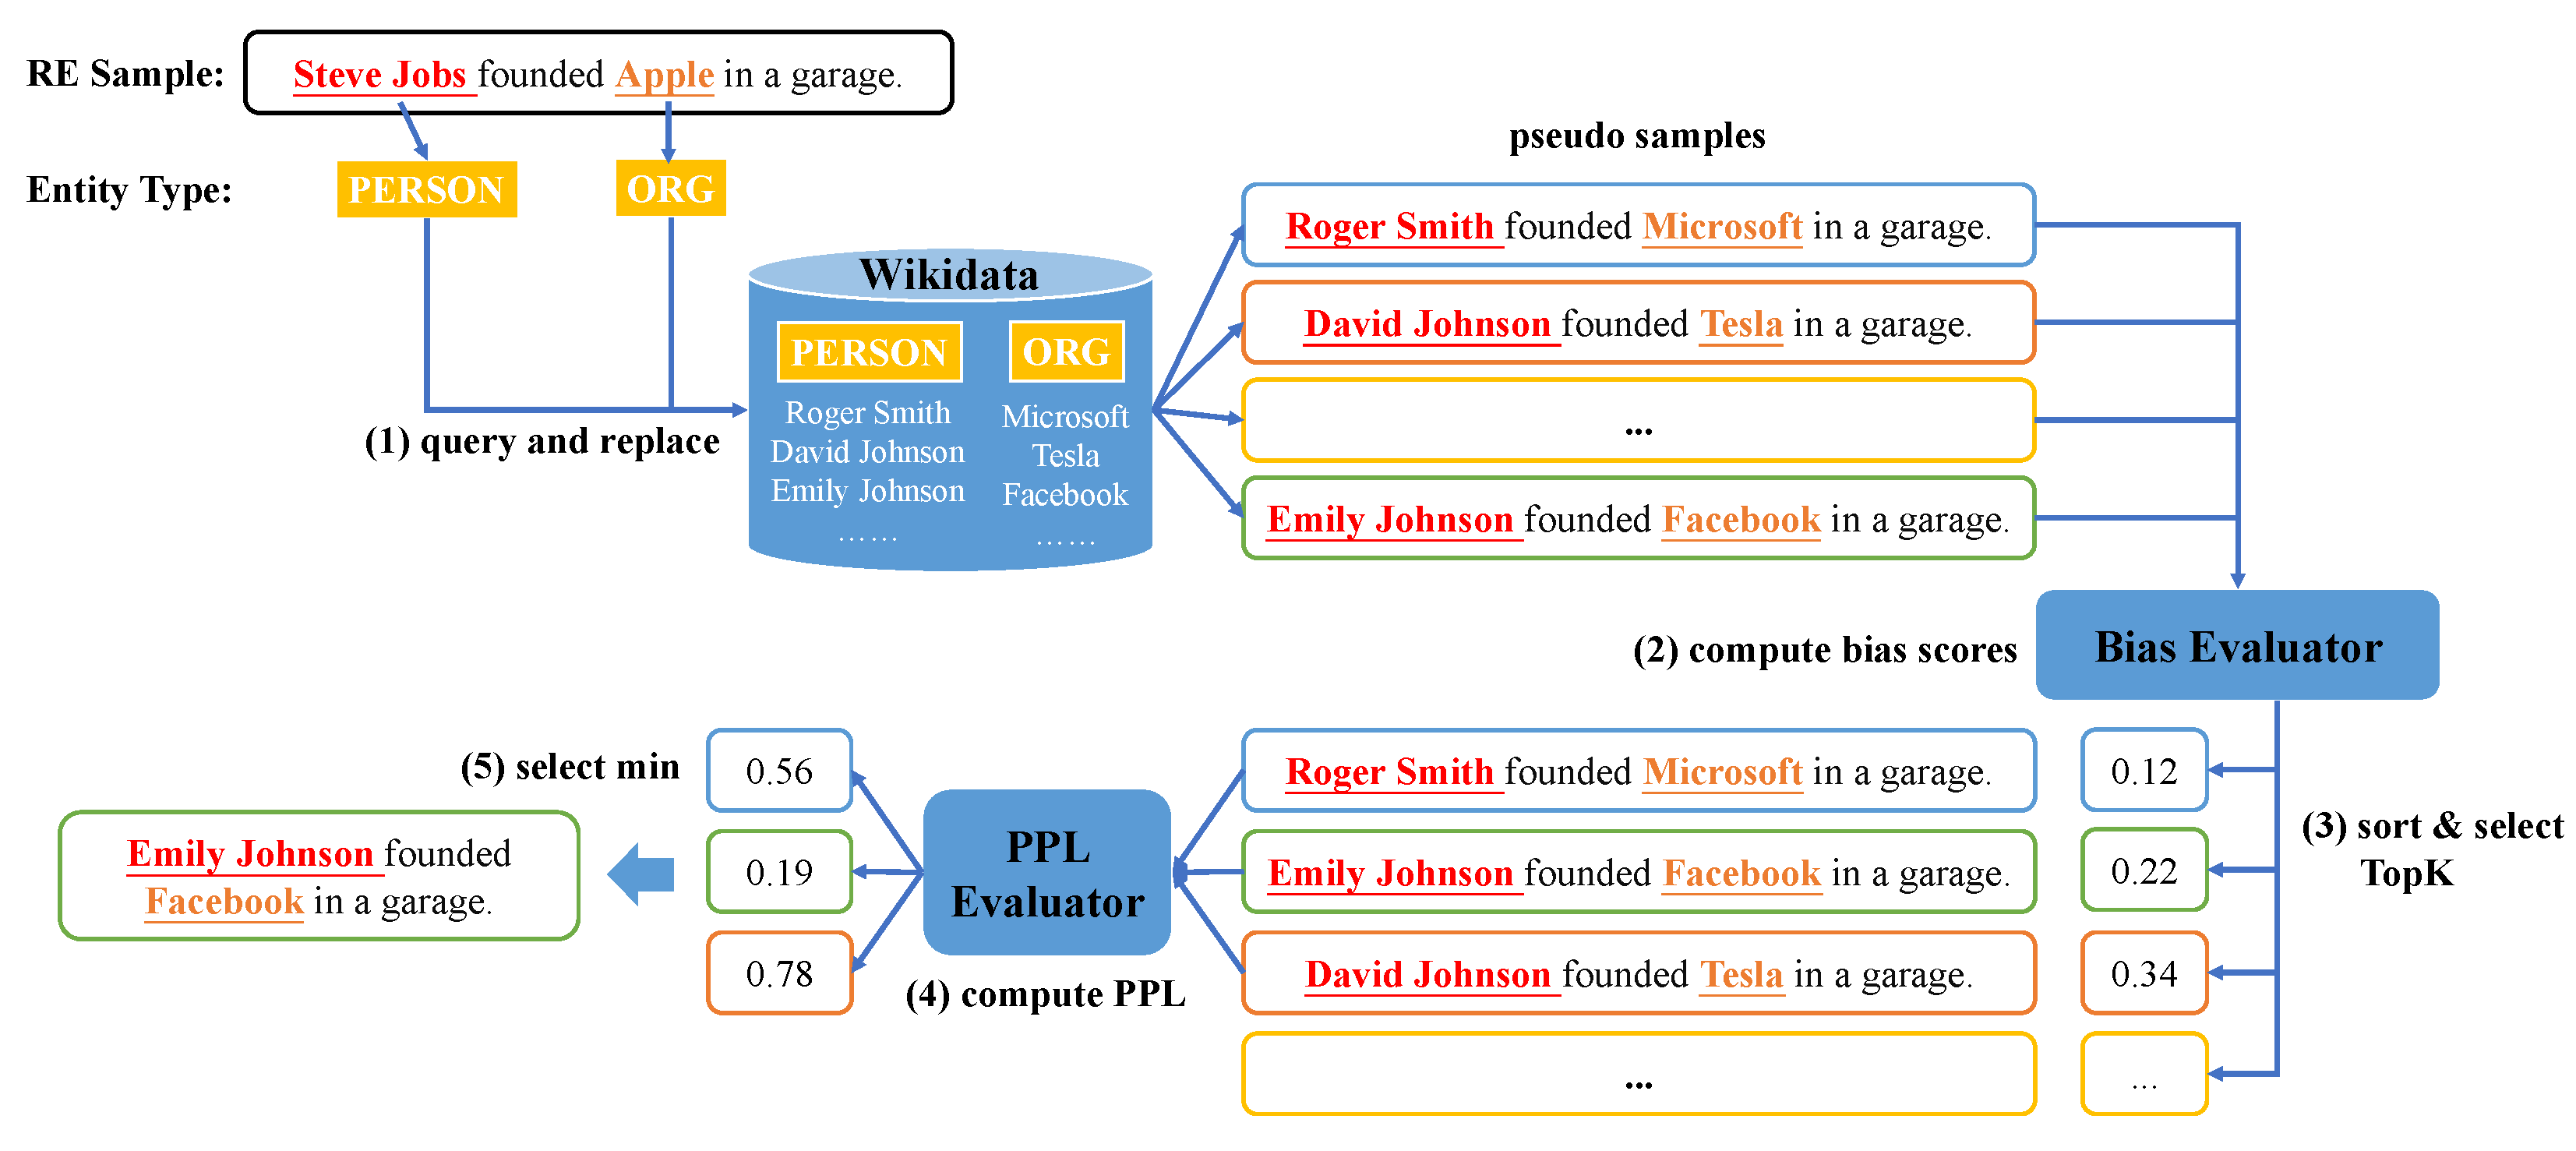
\includegraphics[width=\linewidth]{figure/workflow.pdf}
    \caption{The construction workflow of DREB benchmark.}
    \label{fig:workflow}
\end{figure*}

%We introduce a debiased relation extraction benchmark DREB tailored to address entity bias, with the goal of dismantling the pseudo-correlations between entity mentions and relation types, thus preventing relation extraction models from merely inferring relations based on entity mentions. As depicted in Figure \ref{fig:workflow}, DREB construction involves processing the test set's relation extraction instances, utilizing the extensive entity repository of Wikidata \cite{vrandevcic2014wikidata} to identify and substitute entities of the same type as the originals, finally generate the pseudo samples. What sets our method apart is the incorporation of a Bias Evaluator and a PPL evaluator during the substitution phase. Bias Evaluator assesses the entity bias in the pseudo samples, selecting replacements with minimal bias to disrupt the pseudo-correlation between entity mentions and relation types. PPL Evaluator ensures the naturalness and quality of the pseudo samples. The process encompasses two key components: the Bias Evaluator and the PPL Evaluator, which are detailed as follows:

We introduce DREB, a debiased relation extraction benchmark designed to dismantle pseudo-correlations between entity mentions and relation types, preventing models from solely inferring relations based on entity mentions. As illustrated in Figure \ref{fig:workflow}, DREB construction involves substituting entities in the test set with entities of the same type from Wikidata \cite{vrandevcic2014wikidata} to generate pseudo samples. Our method uniquely incorporates a Bias Evaluator to select replacements with minimal bias and a PPL Evaluator to ensure the naturalness and quality of the pseudo samples.

\subsubsection{Bias Evaluator.}
Bias is fundamentally a pseudo-correlation between biased dataset features and their corresponding labels. To counter this, we employ a neural network to model these correlations directly. Given a sample denoted by \( x \) and its corresponding label \( y \), the process of extracting bias features from \( x \) is represented by \( \phi(x) \). By training the network \( F : \phi(x) \rightarrow y \), the output \( F(\phi(x)) \) reflects the bias inherent in \( x \). For entity bias specifically, the feature extraction process \( \phi \) is defined such that it captures the essence of the entity bias present in relation extraction samples. For instance, \( \phi(\text{"Steve Jobs founded Apple in a garage."}) \) would yield "Steve Jobs" and "Apple." We preprocess the relation extraction training set \( \mathcal{D} \) with \( \phi(x) \) to construct a synthetic dataset \( \mathcal{D}_{\text{EntityBias}} \), which allows us to model the entity bias directly. The resulting model, once trained, serves as a bias evaluator to measure the degree of entity bias in pseudo samples.

\subsubsection{PPL Evaluator.}
Entity replacement schemes generate synthetic text data, which may result in some degree of unnaturalness. To improve the quality of the challenge set, we generate multiple synthetic samples in batches and use GPT-2 \cite{radford2019language} as a language model to calculate the perplexity of these samples. Given a sequence \( \mathbf{W} = (w_1, w_2, \ldots, w_n) \), where \( w_i \) is the \( i \)-th word and \( n \) is the number of words in the sequence, the perplexity can be calculated using the following formula:

\begin{equation}
    \begin{aligned}
        \log \text{PPL}(W) &= \log \left( \frac{1}{P(w_1, w_2, \ldots, w_n)} \right)^{\frac{1}{n}} \\
        &= -\frac{1}{n} \sum_{i=1}^{n} \log P(w_i|w_1, \ldots, w_{i-1})
    \end{aligned}
\end{equation}

\noindent where \( P(w_1, w_2, \ldots, w_n) \) is the probability of the sequence \( \mathbf{W} \). We then select the sample with the lowest perplexity as the final generated sample. Through this process, we can filter out the most natural samples according to the language model, thus enhancing the naturalness and overall quality of the challenge set.

We selected widely used relation extraction datasets TACRED, TACREV, and Re-TACRED and applied our proposed debiasing dataset construction strategy to build DREB benchmark. These datasets belong to the sentence-level relation extraction category, where TACRED is the initial version, TACREV is a revised version that addresses annotation and noise issues in the test and validation sets of TACRED, and Re-TACRED redesigns the relation types and the dataset itself.

\subsection{Benchmark Analysis}

\subsubsection{Does DREB introduce distribution biases?}
Figure \ref{fig:distribution_bias} compares the relation distributions between DREB, the original datasets, and the method by \cite{wang2022should}. It shows that the datasets constructed by \cite{wang2022should}'s method exhibit significant shifts in relation distribution compared to the original datasets, particularly with a notable reduction in the proportion of \textbf{no\_relation}. This suggests that models could simply lower their classification thresholds to boost recall, artificially inflating evaluation metrics. In contrast, DREB maintains identical relation distributions to the original datasets, avoiding the introduction of new distribution biases and ensuring the accurate assessment of debiasing methods.
%Figure \ref{fig:distribution_bias} shows the comparison of relation distributions between the DREB, original datasets and \cite{wang2022should}'s method. It can be observed that the datasets constructed by \cite{wang2022should}'s method exhibit significant shifts in relation distribution compared to the original datasets. Specifically, the proportion of \textbf{no\_relation} is notably reduced, implying that models could simply lower their classification thresholds to increase recall, thereby improving evaluation metrics. In contrast, DREB maintains identical relation distributions to the original datasets, thus avoiding the introduction of new distribution biases, which ensures the accurate assessment of debiasing methods.

\begin{figure}[ht]
    \centering
    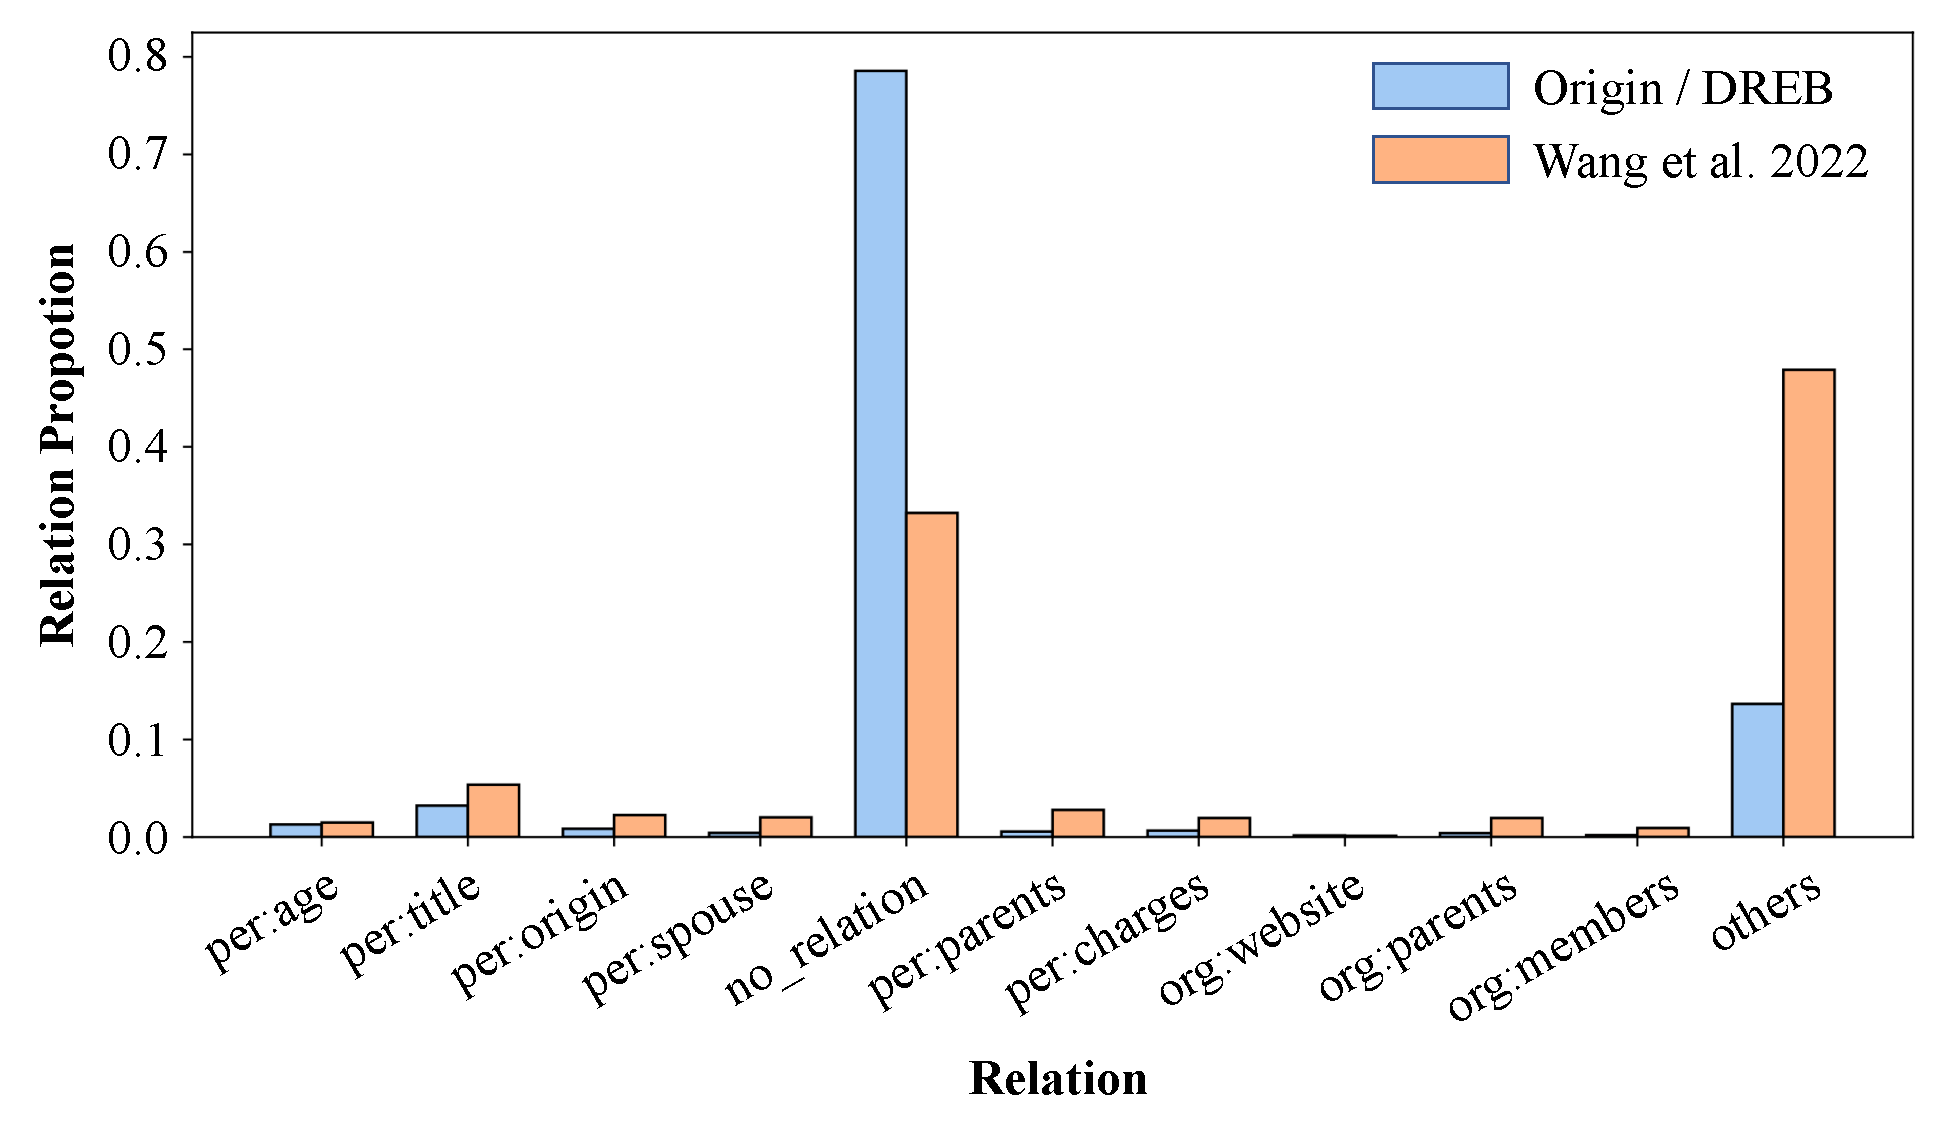
\includegraphics[width=\linewidth]{figure/distribution_bias.pdf}
    \caption{Comparison of relation type distributions.}
    \label{fig:distribution_bias}
\end{figure}

\subsubsection{Does DREB introduce semantic biases?}
We compared the semantic distribution differences between DREB test set samples generated with and without the PPL Evaluator (w/ and w/o PPL Evaluator, respectively) and the original test set samples. As shown in Figure \ref{fig:semantic_bias}, we used SBERT \cite{reimers2019sentence} to encode the samples into feature vectors and then applied PCA \cite{smith2002tutorial} to reduce them to a 2D space for visualization. Without the PPL Evaluator, there was a noticeable distribution shift in the generated samples compared to the original samples, introducing semantic bias. However, when the PPL Evaluator was used, the generated samples largely overlapped with the original samples, avoiding the introduction of semantic bias. This visualization demonstrates that the PPL Evaluator effectively maintains the continuity of samples in the semantic space during the generation of DREB samples, ensuring their semantic naturalness and consistency with the original dataset samples.
%We compared the semantic distribution differences between DREB test set samples generated with and without the PPL Evaluator (w/ and w/o PPL Evaluator, respectively) and the original test set samples. As shown in Figure \ref{fig:semantic_bias}, we used SBERT \cite{reimers2019sentence} to encode the samples to obtain their feature vectors and then applied PCA \cite{smith2002tutorial} to reduce them to a 2D space for visualization. We observed that without using the PPL Evaluator, there was a noticeable distribution shift in the samples of the dataset compared to the original samples, introducing semantic bias. However, when the PPL Evaluator was used, the samples in the dataset largely overlapped with the original samples, avoiding the introduction of semantic bias. This visualization demonstrates that the PPL Evaluator effectively maintains the continuity of samples in the semantic space during the generation of DREB samples, ensuring the semantic naturalness of DREB and keeping them consistent with the original dataset samples.

\begin{figure}[ht]
    \centering
    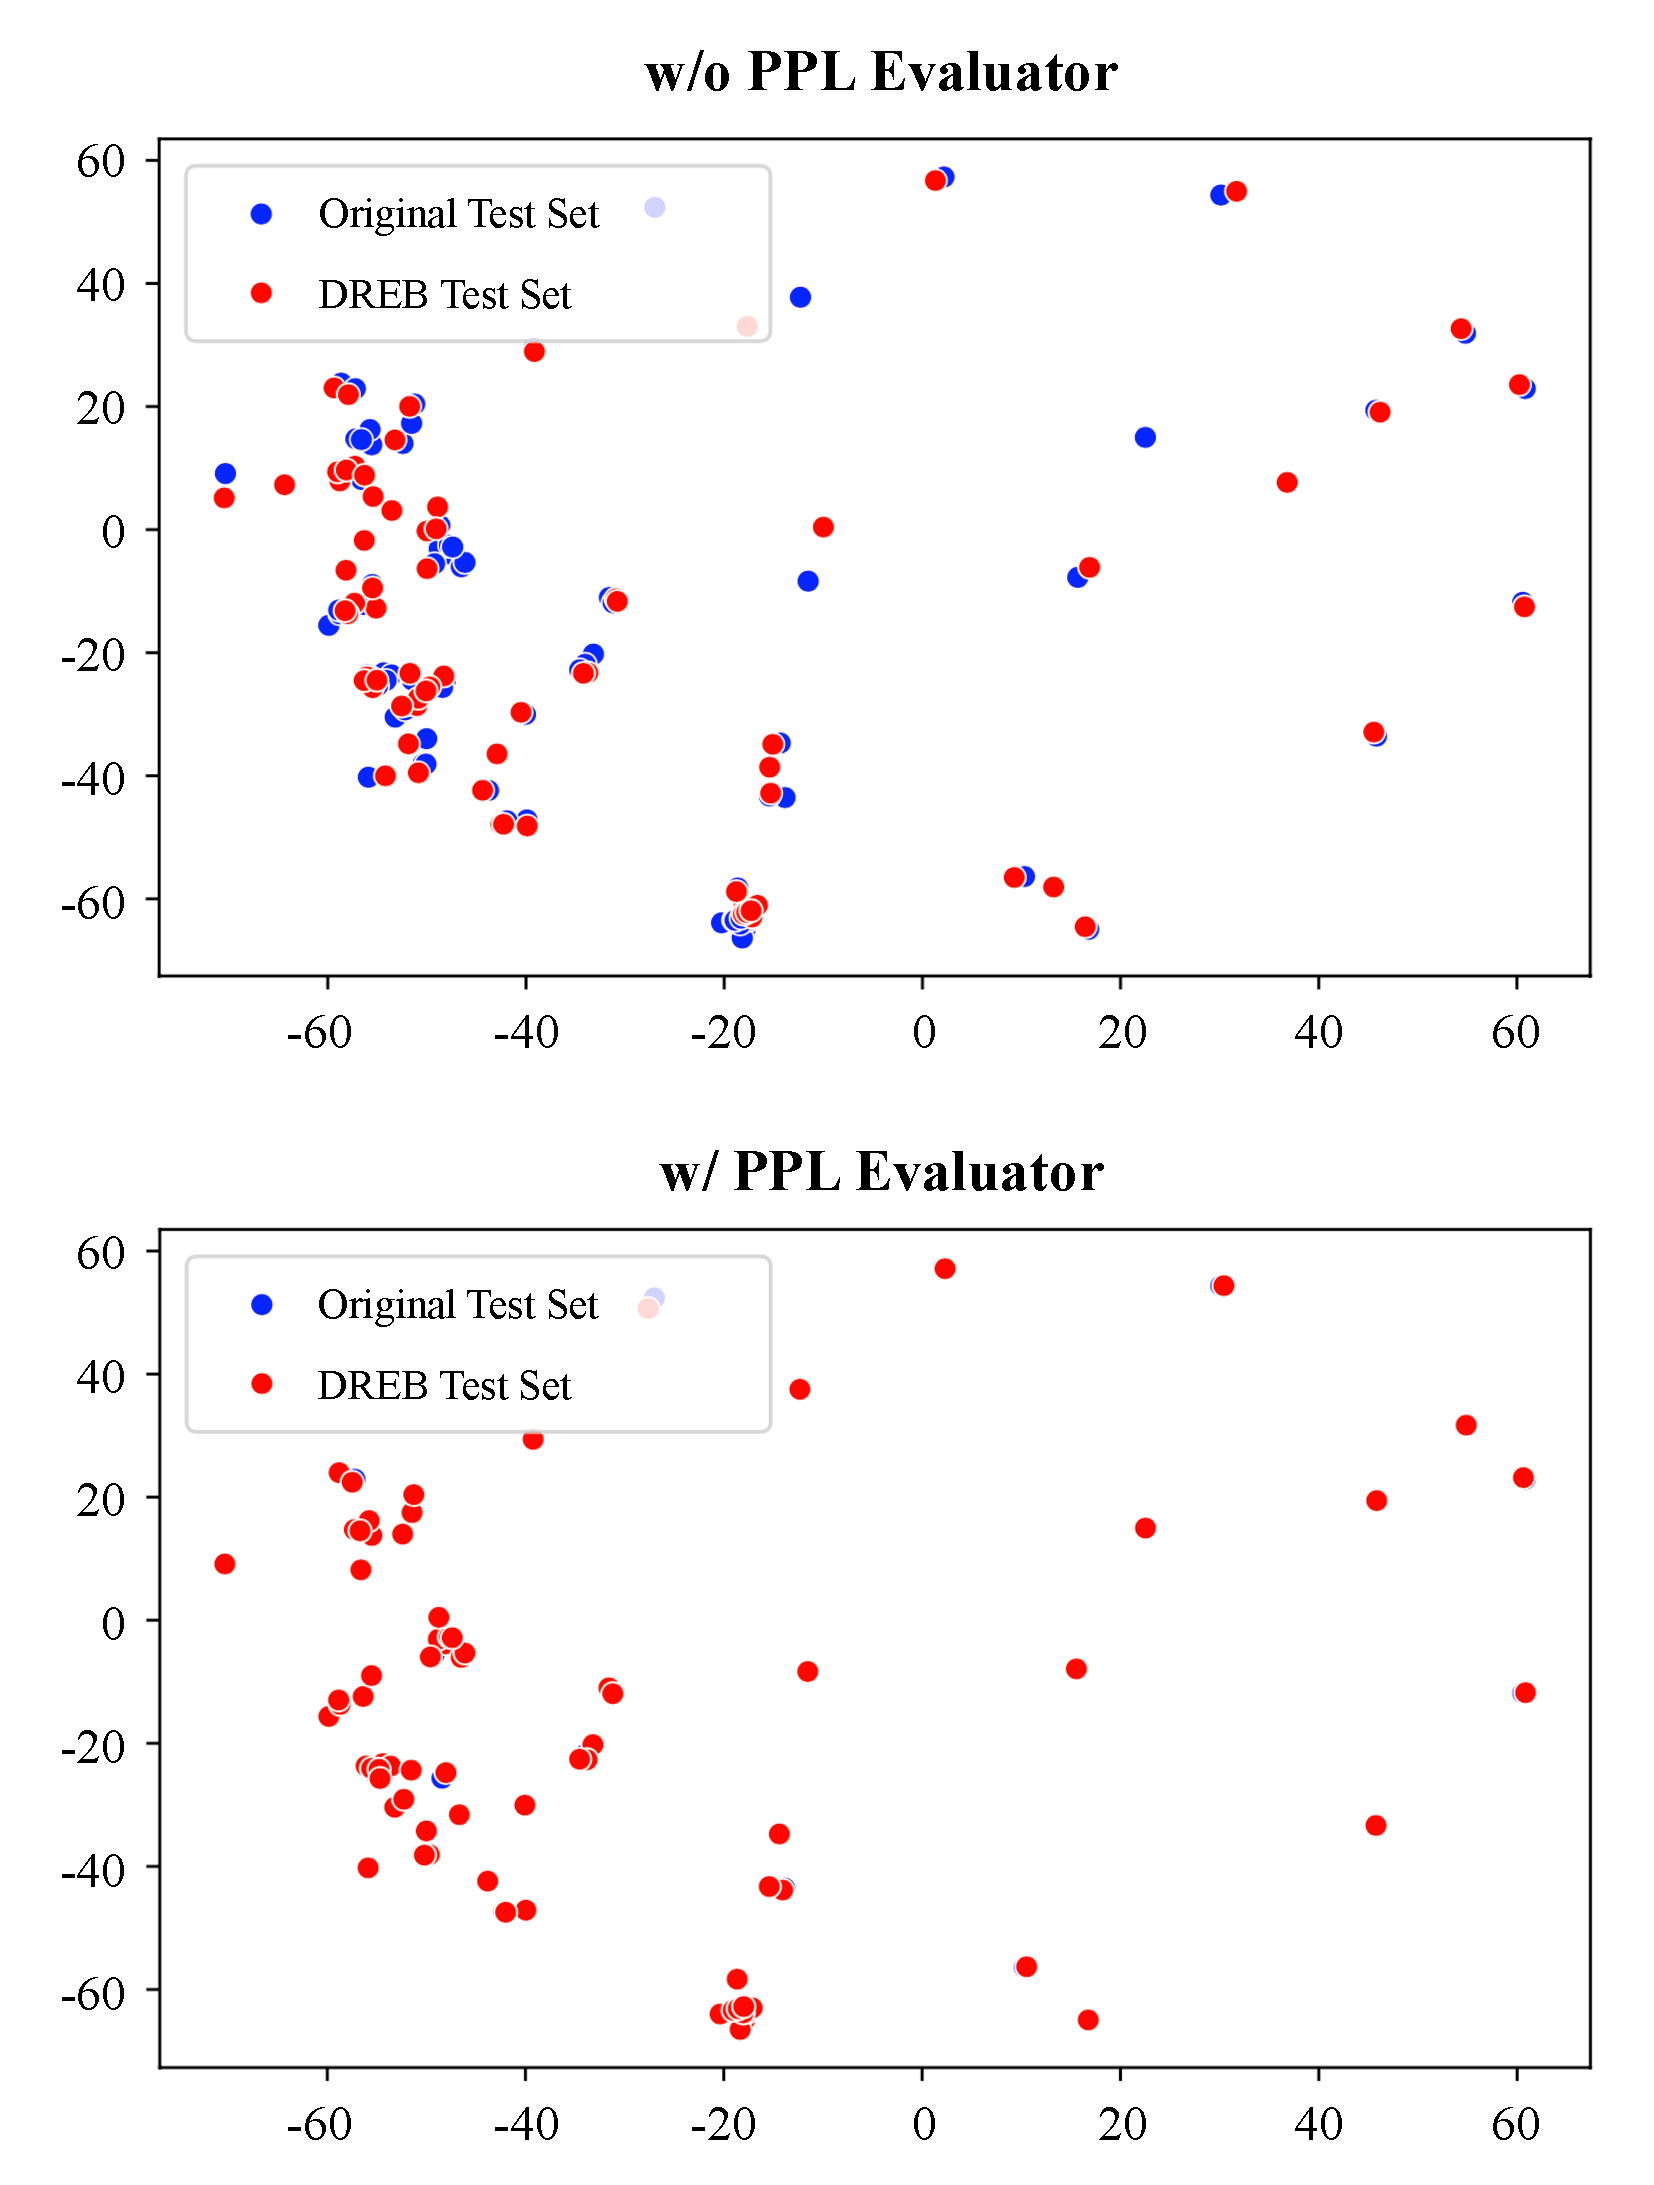
\includegraphics[width=\linewidth]{figure/semantic_bias.pdf}
    \caption{Comparison of semantic distributions. The PPL Evaluator can effectively control semantic bias.}
    \label{fig:semantic_bias}
\end{figure}





\section{MixDebias: A New Baseline on DREB}

\begin{figure*}[ht]
    \centering
    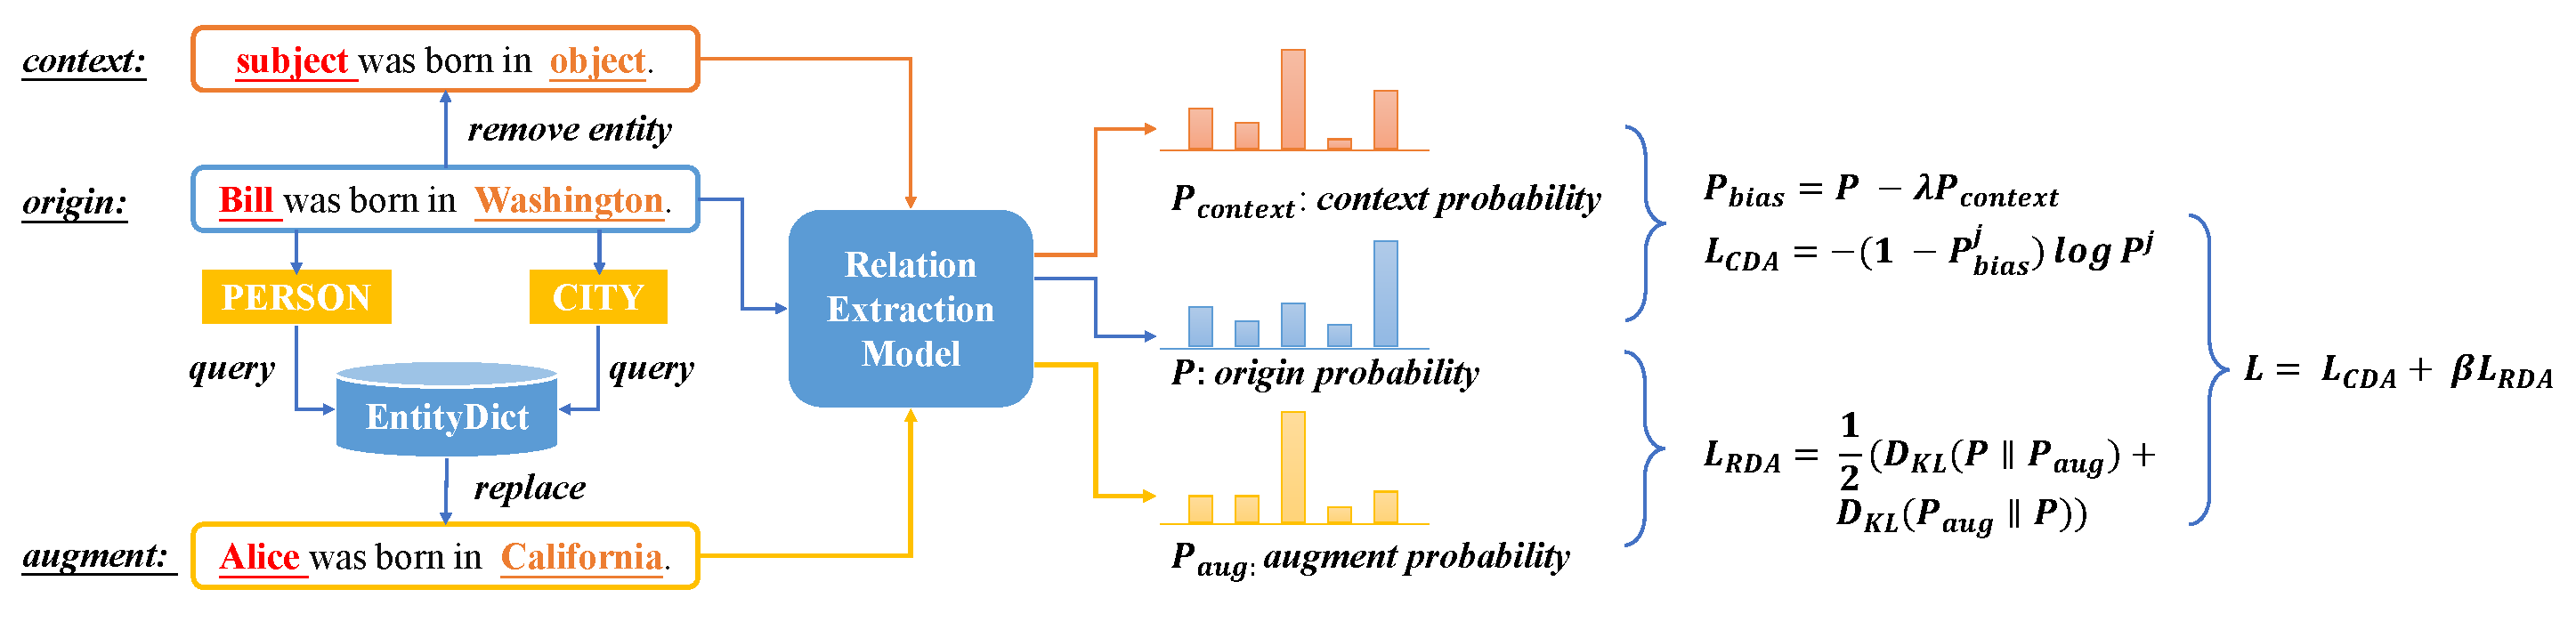
\includegraphics[width=\linewidth]{figure/mixdebias.pdf}
    \caption{The overall workflow of MixDebias.}
    \label{fig:mixdebias}
\end{figure*}

Based on the DREB, we also introduce a method called MixDebias as a new baseline, which debiases from both the data and model training levels (Figure \ref{fig:mixdebias}).

\subsubsection{Data-level debiasing (RDA, Regularized Debias Approach):} 
Entity mentions, despite their potential to cause bias, are valuable as they can prevent ambiguity, particularly in sentences with multiple entities of the same type. Instead of simplistically substituting entities with their corresponding entity types, we propose an approach that generates multiple data-augmented samples from an original training sample through entity replacement. This process is guided by a Kullback-Leibler Divergence (KL Divergence) constraint that encourages the model to produce probability distributions \( P \) and \( P_{aug} \) that are as similar as possible when presented with the original and augmented samples, respectively. We term this KL divergence constraint \( \mathcal{L}_{RDA} \), and its incorporation effectively reduces the model's reliance on the entities present in the input, thereby enhancing the model's generalization capabilities.

Specifically, we construct an entity dictionary (EntityDict) by extracting entities from the training set, facilitating the dynamic creation of data-augmented samples during training through entity replacement. We deliberately avoid sourcing entities from external resources like Wikidata for augmentation to prevent the introduction of lexical bias during the training phase. Throughout training, for an original sample, we dynamically retrieve entities of the same type from the EntityDict and generate a new data-augmented sample via entity replacement. Both the original and augmented samples are then fed into the relation extraction model, yielding two probability distributions, \( P \) and \( P_{aug} \). We calculate the KL divergence between these distributions. Due to the asymmetry of KL divergence, we calculate \(D_{KL}(P || P_{aug})\) and \(D_{KL}(P_{aug} || P)\) and average them to get \(\mathcal{L}_{RDA}\).

\subsubsection{Model-level debiasing (CDA, Casual Debias Approach):}
The CDA method identifies and quantifies entity bias through causal effect estimation and uses this estimation to guide model training, reducing the model's dependence on input features that may lead to bias. In causal effect estimation, we try to understand how different factors affect the results, especially how other variables affect the results when some variables are controlled. For relation extraction models, causal effects can be used to identify and reduce the model's dependence on input features that may have pseudo-correlation with the target output, rather than real causal relationships. The CDA method uses causal effect estimation to build a bias model (Bias Model), which assesses the degree of entity bias in each sample. Specifically, by providing only the context input to the model to obtain the probability distribution \( P_{context} \), and the original sample input to the model to obtain the probability distribution \( P \), then calculate \( P - \lambda P_{context} \) to obtain the bias probability distribution \( P_{bias} \), where \( \lambda \) is a hyperparameter. This bias probability distribution reflects the degree of entity bias in the sample. The CDA method uses Debiased Focal Loss \cite{mahabadi2020end} for model training, which adjusts the model's predictions using the bias probability, thereby reducing the model's dependence on entity mentions.

\begin{equation}
    \mathcal{L}_{CDA} = -(1 - P_{bias}^j) \log P^j
\end{equation}

\noindent where \( j \) is the correct relation type label. When \( \lambda \) is 0, \( \mathcal{L}_{CDA} \) degenerates into \( -(1 - P^j) \log P^j \), which is the Focal Loss. As a common form of model regularization loss, we modify it with \( P_{context} \) to achieve a debiasing effect. In this way, the CDA method reduces the entity bias learned by the model during the training process, improving the model's generalization ability when facing different entities.

Finally, we introduce a hyperparameter \( \beta \) to combine \( \mathcal{L}_{RDA} \) and \( \mathcal{L}_{CDA} \) in a weighted manner to obtain the final loss function \( \mathcal{L}_{MixDebias} \):

\begin{equation}
    \begin{aligned}
        \mathcal{L}_{MixDebias} &= \mathcal{L}_{CDA} + \beta \mathcal{L}_{RDA} \\
        &= -(1 - P_{bias}^j) \log P^j + \\
        & \quad \frac{\beta}{2} (D_{KL} (P || P_{aug}) + D_{KL} (P_{aug} || P)) \\
        &= - (1 - (P^j - \lambda P_{context}^j)) \log P^j + \\
        & \quad \frac{\beta}{2} (D_{KL} (P || P_{aug}) + D_{KL} (P_{aug} || P))
    \end{aligned}
\end{equation}

\subsection{Evaluation}

\subsubsection{Evaluation metric.}
Consistent with previous work, we adopt the F1-score, which is the harmonic mean of precision and recall, as our primary evaluation metric. Additionally, we designed the Bias Mitigation Efficiency (BME) to comprehensively evaluate the effectiveness of debiasing methods, taking into account both the performance impact on the original dataset and the performance improvement on DREB. Specifically, let $\widetilde{F1}_{\text{origin}}$ and \( \widetilde{F1}_{\text{DREB}} \) be the F1 scores of the baseline model on the original dataset and DREB, respectively. Let \( F1_{\text{origin}} \) and \( F1_{\text{DREB}} \) be the F1 scores of the new model on the original dataset and DREB, respectively. The BME is then calculated as:

\begin{equation}
    \text{BME} = \alpha \cdot \frac{F1_{\text{origin}}}{\widetilde{F1}_{\text{origin}}} + (1 - \alpha) \cdot \frac{F1_{\text{DREB}}}{\widetilde{F1}_{\text{DREB}}}
\end{equation}

\noindent where in our experiments, we set \( \alpha = 0.5 \).

\subsubsection{Baselines.} 
To focus on analyzing the debiasing effects of the model, models that retain entity mentions in the input during the preprocessing stage better meet our needs. We selected \textbf{LUKE} \cite{yamada2020luke} and \textbf{IRE} \cite{zhou2022improved} for this purpose. LUKE is a transformer-based model that introduces a novel pretraining task for learning contextualized representations of both words and entities. IRE introduces typed entity markers that include both the entity spans and their types into the input text, allowing for a more comprehensive representation of entity mentions. In terms of debiasing methods, we primarily chose the following as baseline methods for comparison: \textbf{Focal} \cite{lin2018focal} reduces the model's reliance on entities by attenuating the influence of easily classified samples and amplifying the significance of challenging ones, thereby recalibrating the training focus towards hard-to-classify instances. \textbf{R-Drop} \cite{liang2021r} enhances model generalization by enforcing consistency between output distributions of sub-models created through dropout, processing each mini-batch data sample twice to generate distinct outputs, and minimizing the bidirectional Kullback-Leibler divergence, thereby reducing reliance on entity mentions and improving the model's robustness. \textbf{DFL} \cite{mahabadi2020end} adjusts the loss function using a focusing parameter based on the bias-only model's predictions, effectively reducing the model's dependency on entities by downweighting samples with high entity bias, which enhances the model's robustness and generalization without altering its original architecture. \textbf{PoE} \cite{hinton2002training} employs a unique integration of individual expert models by multiplying their probability distributions, including a biased distribution derived solely from entity inputs, with the model's predictive distribution. This multiplication and subsequent renormalization subtly decrease the influence of samples with significant entity bias, effectively reducing the model's reliance on these entities while optimizing model performance. \textbf{CoRE} \cite{wang2022should} mitigates biases by constructing a causal graph to identify dependencies and using counterfactual scenarios to pinpoint entity biases, subsequently refining predictions through an adaptive bias mitigation process that emphasizes textual context over entity reliance, leading to debiased outcomes.

\subsubsection{Main results.}

Table \ref{table:main} demonstrates the performance comparison of various relation extraction models and different debiasing methods on different datasets, where \( F1_{\text{origin}} \) represents the performance on the original test set, and \( F1_{\text{DREB}} \) represents the performance on DREB benchmark proposed in this paper.

\begin{table*}[ht]
\centering
    \begin{tabularx}{\linewidth}{p{2.9cm}|p{1.2cm}<{\centering}p{1.2cm}<{\centering}p{1.2cm}<{\centering}|p{1.2cm}<{\centering}p{1.2cm}<{\centering}p{1.2cm}<{\centering}|p{1.2cm}<{\centering}p{1.2cm}<{\centering}p{1.2cm}<{\centering}}
    \toprule

    \multirow{2}*{\textbf{Model}} & \multicolumn{3}{c|}{\textbf{TACRED}} & \multicolumn{3}{c|}{\textbf{TACREV}} & \multicolumn{3}{c}{\textbf{Re-TACRED}} \\
    \cmidrule(lr){2-10}
    & $F1_{\text{origin}}$ & $F1_{\text{DREB}}$  & BME & $F1_{\text{origin}}$  & $F1_{\text{DREB}}$  & BME & $F1_{\text{origin}}$  & $F1_{\text{DREB}}$  & BME \\
   
    \midrule
        LUKE & 70.82 & 44.40 & - & 80.16 & 50.60 & - & 88.92 & 39.40 & - \\
        +Focal & 69.94 & 45.55 & 1.01 & 79.15 & 52.48 & 1.01 & 88.58 & 39.32 & 1.00 \\
        +R-Drop & \textbf{70.99} & 46.68 & 1.03 & \textbf{81.06} & 53.85 & 1.04 & \textbf{89.53} & 40.89 & 1.02 \\
        +DFL & 65.04 & 48.48 & 1.01 & 71.31 & 53.17 & 0.97 & 84.15 & 43.94 & 1.03 \\
        +PoE & 63.32 & 47.63 & 0.98 & 68.82 & 52.02 & 0.94 & 82.46 & 44.10 & 1.02 \\
        +CoRE & 70.04 & 47.87 & 1.03 & 79.82 & 54.88 & 1.04 & 87.13 & 41.94 & 1.02 \\
        +MixDebias & 69.93 & \textbf{62.44} & \textbf{1.20} & 80.91 & \textbf{72.93} & \textbf{1.23} & 87.95 & \textbf{77.71} & \textbf{1.48} \\
    \midrule
        IRE & 71.27 & 50.94 & - & 79.36 & 57.20 & - & 87.43 & 46.25 & - \\
        +Focal & 71.11 & 50.97 & 1.00 & 78.55 & 57.51 & 1.00 & 87.51 & 48.22 & 1.02 \\
        +R-Drop & 71.13 & 52.98 & 1.02 & 80.37 & 59.71 & 1.03 & \textbf{87.96} & 48.40 & 1.03 \\
        +DFL & 65.72 & 56.28 & 1.01 & 70.18 & 60.13 & 0.97 & 80.17 & 54.03 & 1.04 \\
        +PoE & 64.72 & 54.67 & 0.99 & 69.12 & 59.28 & 0.95 & 81.35 & 51.41 & 1.02 \\
        +CoRE & 70.43 & 55.00 & 1.03 & 78.82 & 60.81 & 1.03 & 86.21 & 48.36 & 1.02 \\
        +MixDebias & \textbf{71.99} & \textbf{70.02} & \textbf{1.19} & \textbf{80.97} & \textbf{79.15} & \textbf{1.20} & 87.27 & \textbf{82.17} & \textbf{1.39} \\
    \bottomrule
    \end{tabularx}
\caption{The overall evaluation results. MixDebias significantly enhances performance on DREB and achieves comparable performance to the best models on the original dataset. In terms of the comprehensive metric BME, MixDebias also leads far ahead of other baseline methods.}
\label{table:main}
\end{table*}

\begin{table*}[ht]
\centering
    \begin{tabularx}{\linewidth}{p{2.95cm}|p{2cm}<{\centering}p{2cm}<{\centering}|p{2cm}<{\centering}p{2cm}<{\centering}|p{2cm}<{\centering}p{2cm}<{\centering}}
    \toprule

    \multirow{2}*{\textbf{Model}} & \multicolumn{2}{c|}{\textbf{TACRED}} & \multicolumn{2}{c|}{\textbf{TACREV}} & \multicolumn{2}{c}{\textbf{Re-TACRED}} \\
    \cmidrule(lr){2-7}
    & $F1_{\text{origin}}$  & $F1_{\text{DREB}}$ & $F1_{\text{origin}}$  & $F1_{\text{DREB}}$ & $F1_{\text{origin}}$  & $F1_{\text{DREB}}$ \\
   
    \midrule
        LUKE+MixDebias & 69.93 & 62.44 & 80.91 & 72.93 & 87.95 & 77.71 \\
        -CDA & 69.66(-0.27) & 62.06(-0.38) & 80.63(-0.28) & 71.99(-0.94) & 88.45(+0.50) & 78.26(+0.55) \\
        -RDA & 69.68(-0.25) & 45.77(-16.67) & 79.32(-1.59) & 51.91(-21.02) & 88.69(+0.74) & 39.72(-37.99) \\
    \midrule
        IRE+MixDebias & 71.99 & 70.02 & 80.97 & 79.15 & 87.27 & 82.17 \\
        -CDA & 71.92(-0.07) & 70.21(+0.19) & 80.78(-0.19) & 78.60(-0.55) & 87.19(-0.08) & 82.08(-0.09) \\
        -RDA & 71.33(-0.66) & 52.60(-17.42) & 79.36(-1.61) & 58.48(-20.67) & 87.87(+0.60) & 48.22(-33.95) \\
    \bottomrule
    \end{tabularx}
\caption{The ablation study results for the MixDebias method, detailing the performance impacts of individual components CDA and RDA.}
\label{table:ablation}
\end{table*}

%From the experimental results, we can draw the following conclusions: \textbf{LUKE and IRE} both exhibited a significant performance drop on DREB, indicating that their excellent performance on the original test set was partly reliant on entity mentions, which was replaced or obscured in DREB, leading to decreased performance. \textbf{Focal and R-Drop}, while not specifically designed to address entity bias, still contribute to reducing it. These methods, generally aimed at preventing overfitting, have a secondary effect of mitigating the influence of entity mentions on the model's predictions. This suggests that techniques aimed at improving model generalization can indirectly assist in reducing entity bias. \textbf{DFL and PoE}, as specialized debiasing methods, have significantly improved the model's performance on DREB by introducing bias assessment and adjustment mechanisms during the model training process. However, this improvement appears to come at the cost of performance on the original dataset. \textbf{CoRE}, a debiasing method specifically designed to address entity bias, not only enhances the model's performance on DREB but also maintains the model's performance on the original dataset, demonstrating good balance and effective correction of entity bias. Overall, the \textbf{MixDebias} method we proposed has not only shown significant performance improvement on DREB but also preserved or enhanced performance on the original dataset, demonstrating strong adaptability and debiasing effects.

The experimental outcomes yield these insights: \textbf{LUKE and IRE} experienced a notable decline in performance on the DREB, suggesting their initial high results were partially due to reliance on entity mentions that were either removed or disguised in the DREB context, thereby affecting their efficacy. \textbf{Focal and R-Drop}, though not originally intended to tackle entity bias, have still been found to alleviate it. These techniques, primarily targeting overfitting, incidentally lessen the models' dependency on entity cues, indicating that generalization-focused strategies can also indirectly benefit bias reduction. \textbf{DFL and PoE}, as targeted debiasing approaches, markedly bolstered model performance on DREB through the incorporation of bias evaluation and adjustment within the training regime. However, this enhancement seems to have compromised the models' performance on the original data. \textbf{CoRE}, tailored to counteract entity bias, successfully improved DREB performance without sacrificing the original dataset's results, reflecting a balanced and potent debiasing approach. In sum, our proposed \textbf{MixDebias} method has impressively uplifted performance on DREB while also maintaining or even enhancing the original dataset's performance, showcasing its robust adaptability and debiasing capabilities.


\begin{figure*}[ht]
    \centering
    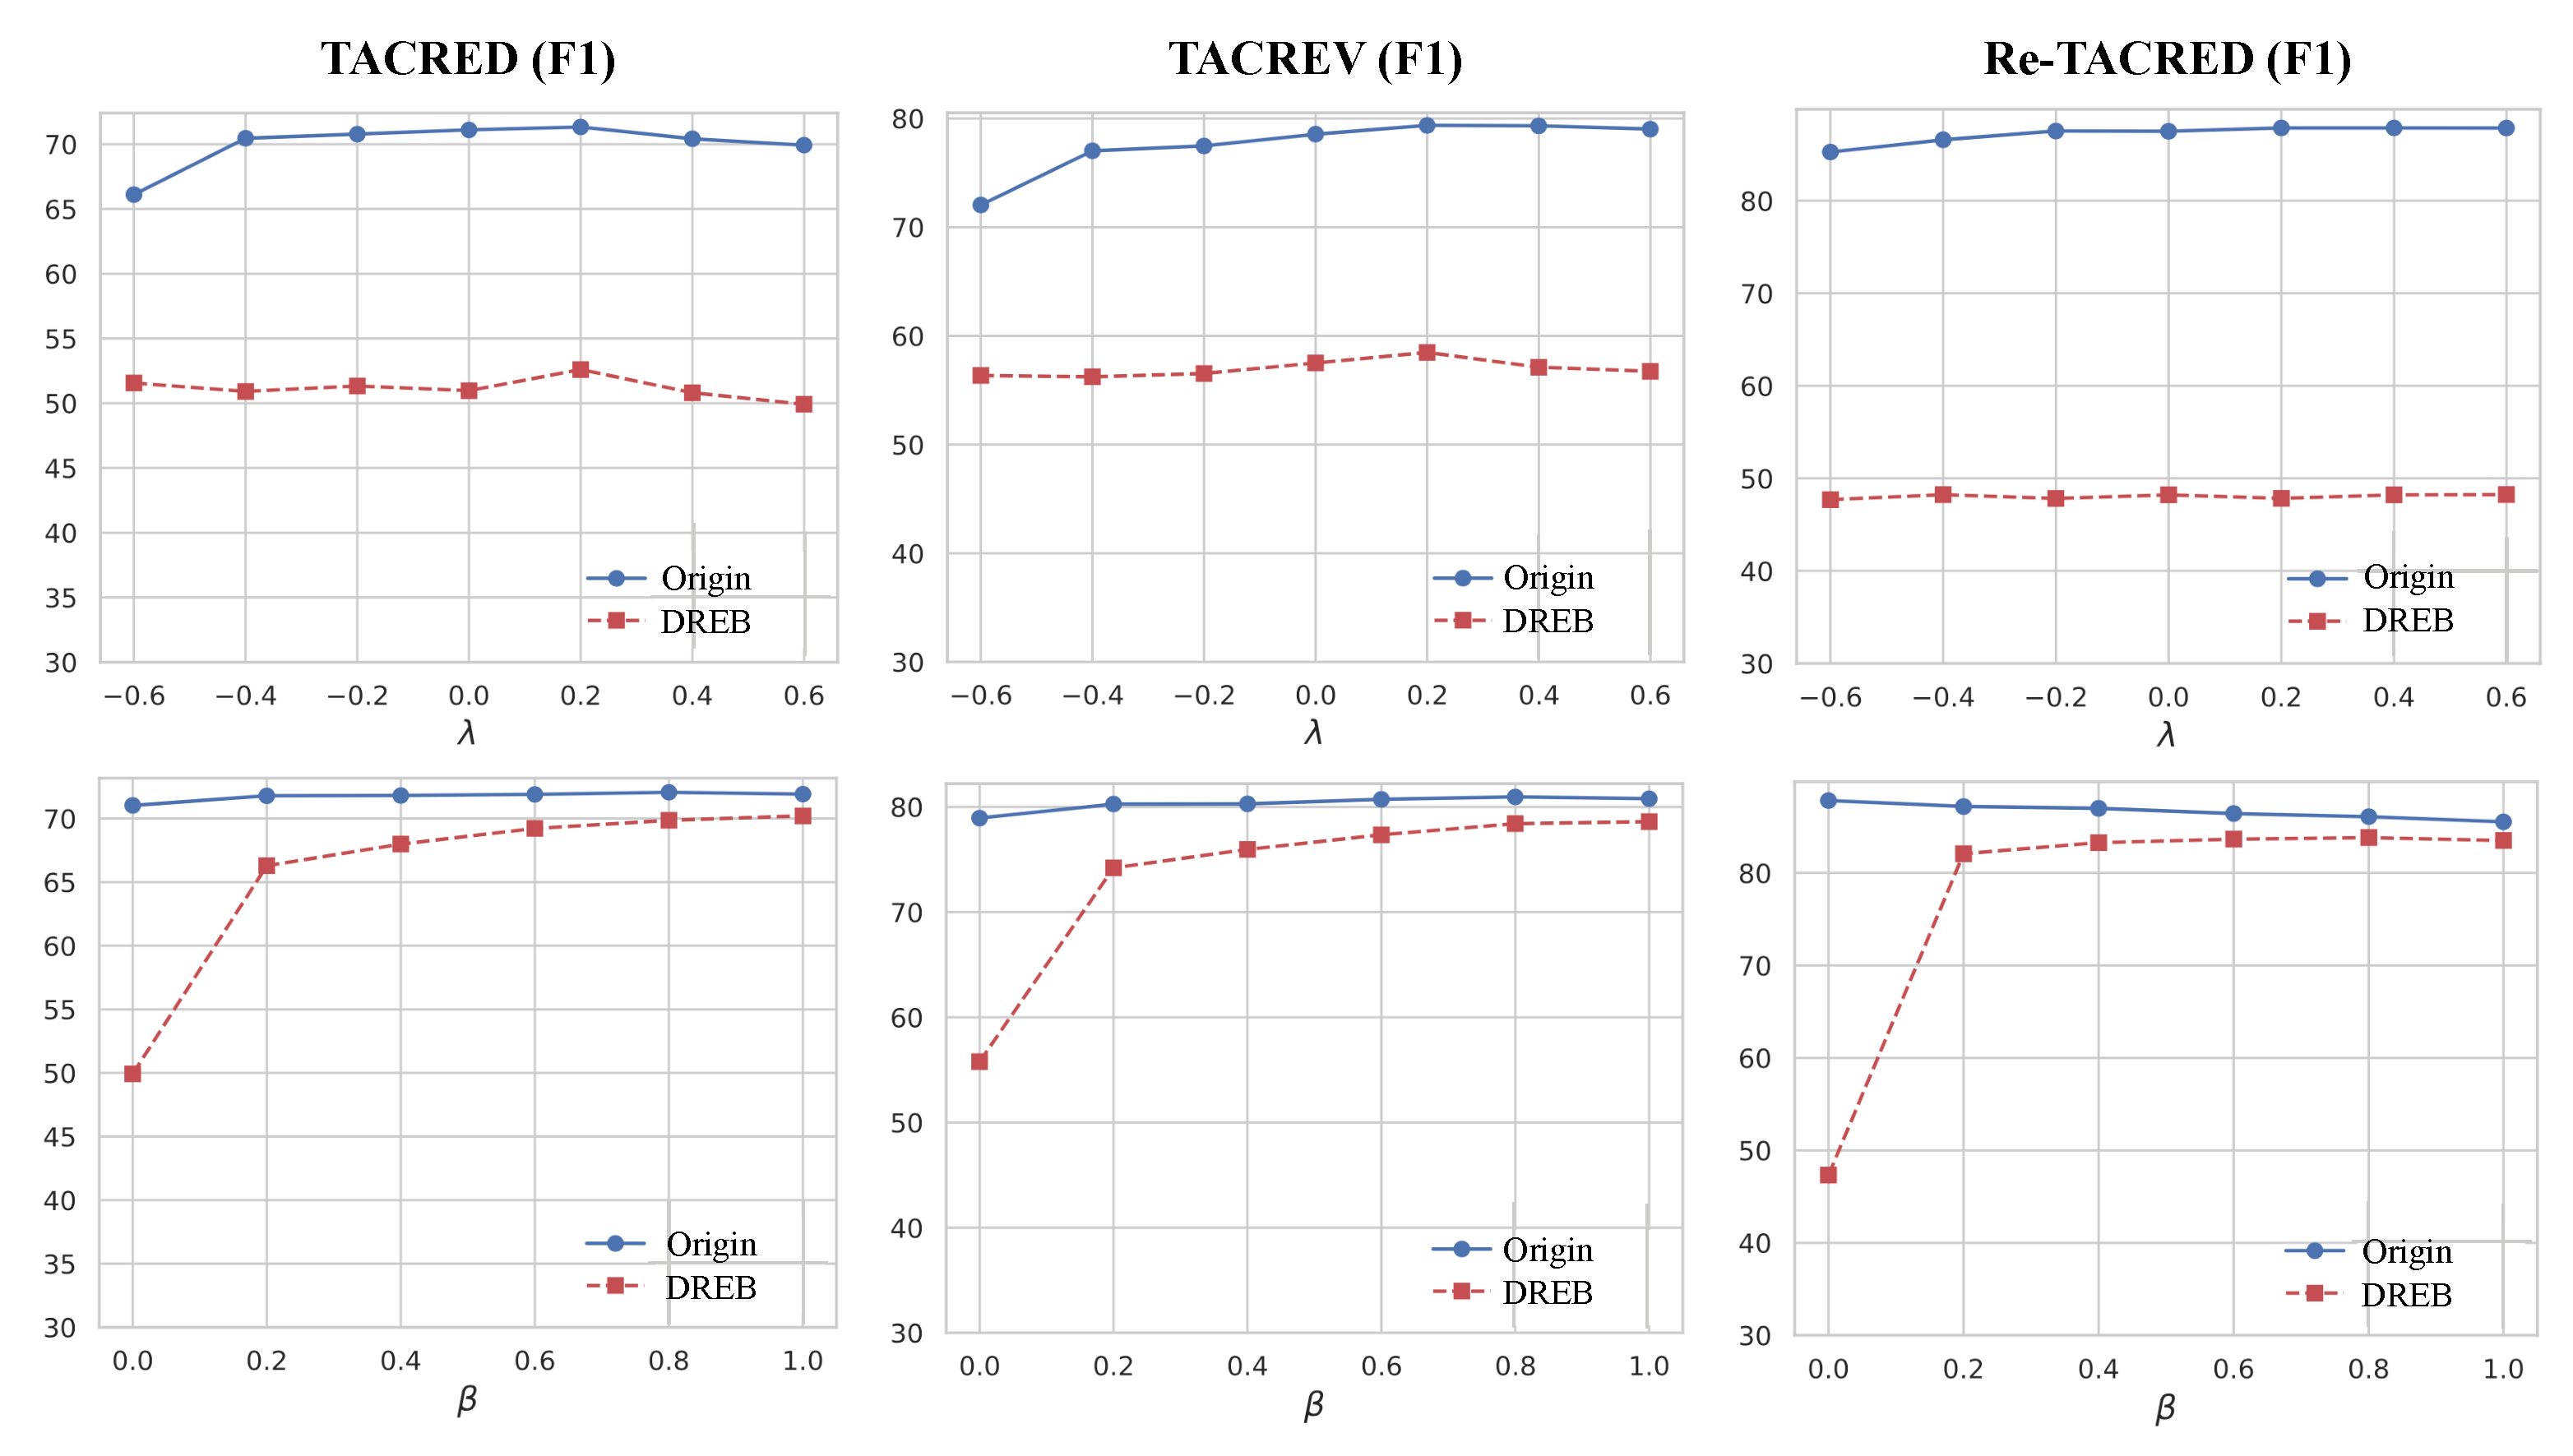
\includegraphics[width=\linewidth]{figure/parameter.pdf}
    \caption{The detailed ablation analysis on the hyperparameters \( \lambda \) and \( \beta \) in MixDebias.}
    \label{fig:parameter}
\end{figure*}

\begin{figure*}[!]
    \centering
    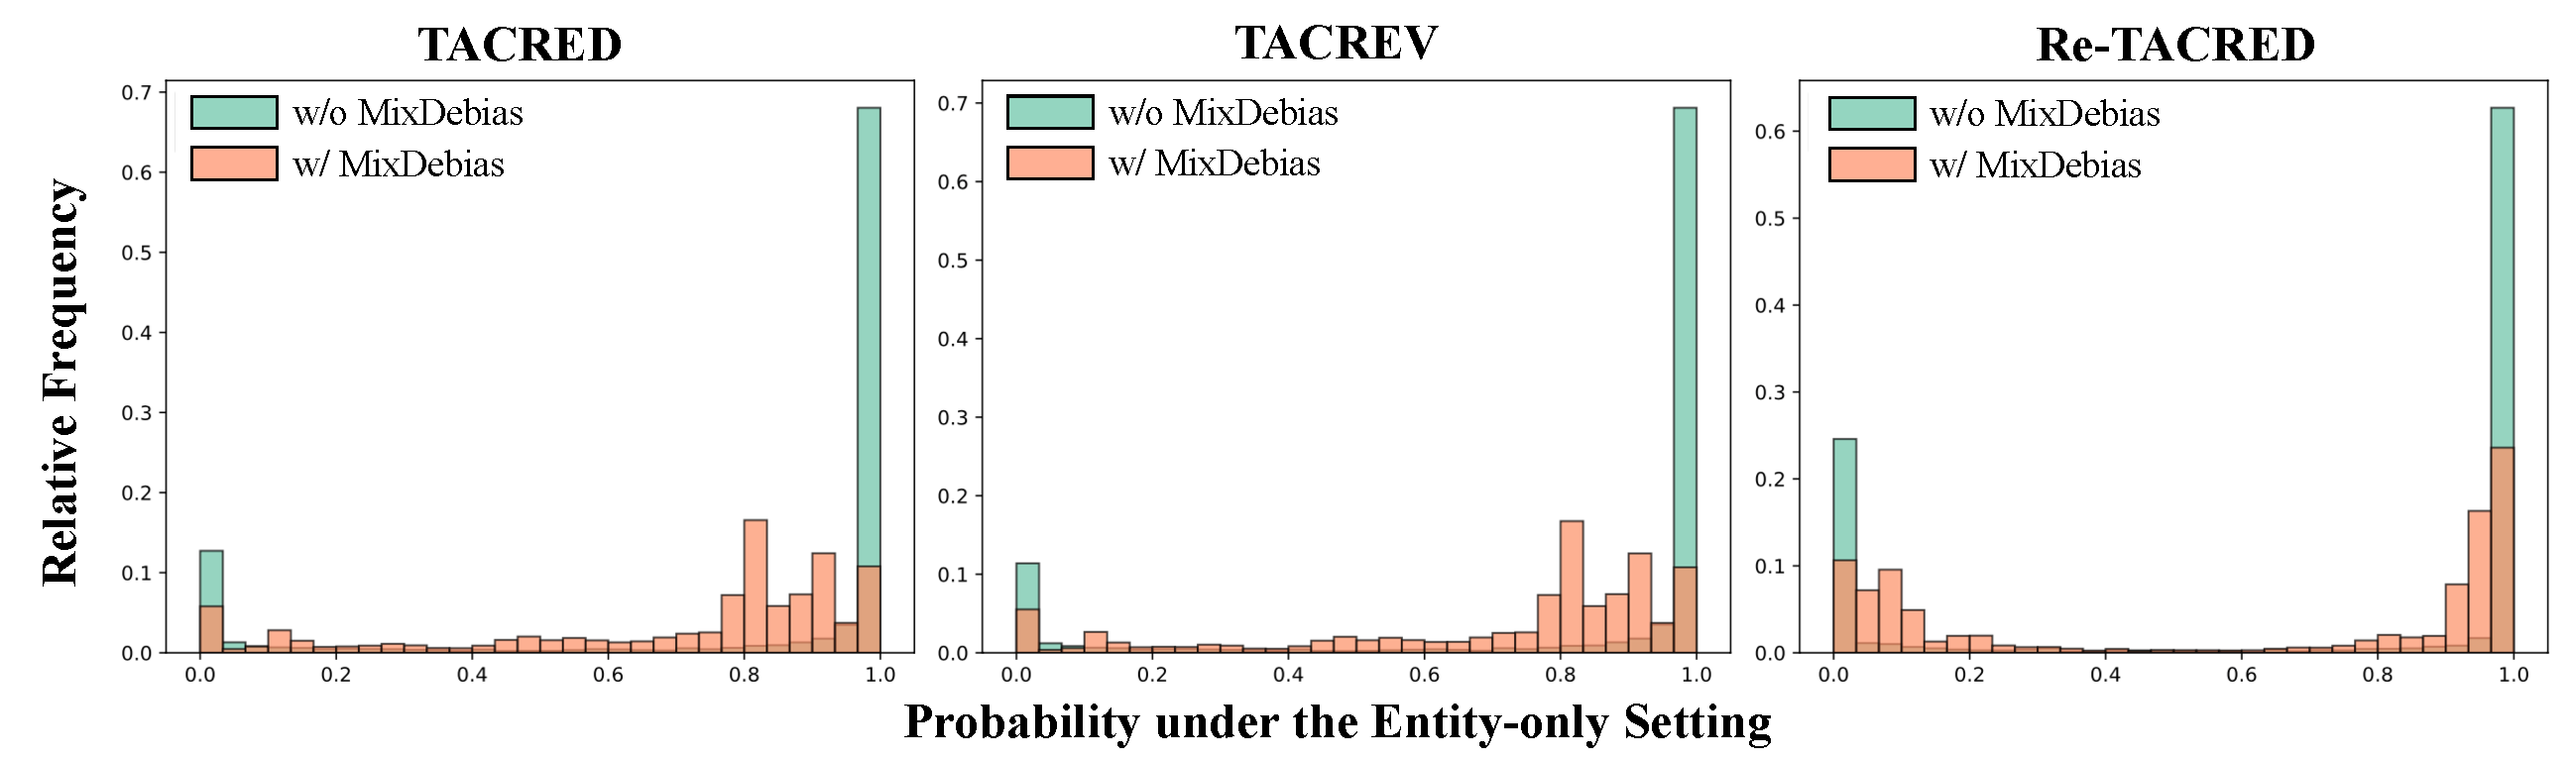
\includegraphics[width=\linewidth]{figure/generalization.pdf}
    \caption{The visualization of debiasing effect. The substantial reduction in model reliance on entity mentions with MixDebias leads to a more uniform probability distribution.}
    \label{fig:generalization}
\end{figure*}

\subsubsection{Ablation study.}

As shown in Table \ref{table:ablation}, we conducted an ablation study on the two components of MixDebias, RDA and CDA. From the experimental results, we can draw the following conclusions: Both RDA and CDA are effective methods for removing entity bias. Overall, RDA is more effective than CDA. However, in most scenarios, these two methods are complementary and can enhance performance on DREB while minimizing the impact on the performance of the original dataset.

% ablation table

At the same time, we conducted a more detailed ablation analysis on the hyperparameters \( \beta \) and \( \lambda \) in MixDebias. Here, \( \beta \) represents the weight of the KL divergence, with a value range of [0.0, 1.0]; and \( \lambda \) represents the hyperparameter for estimating the biased probability distribution of samples using causal effects, with a value range of [-0.6, 0.6]. From Figure \ref{fig:parameter}, we can draw the following conclusions: When \( \beta = 0 \), it is equivalent to the model not considering RDA. However, when \(\beta \neq 0\), introducing RDA leads to significant performance improvements, and as \(\beta\) increases, the debiasing effect becomes stronger. Particularly on noisy datasets such as TACRED and TACREV, the model also shows a slight performance improvement on the original dataset. Compared to \(\beta\), the \(\lambda\) parameter has a smaller impact on model performance. When \(\lambda = 0.2\), the model performs optimally. This suggests that after applying the RDA method, the level of entity bias in the samples is already significantly reduced. In this case, CDA mainly addresses the bias that is difficult to correct at the data level, serving as a complementary effect to RDA, thereby further reducing the model's reliance on entities.

\subsubsection{Model generalization analysis.}

As shown in Figure \ref{fig:generalization}, we plotted the label probability distribution of the model under the setting of entity-only input in the original test set before and after debiasing on the TACRED, TACREV, and Re-TACRED datasets. The experimental results show that for the baseline relation extraction model, under the entity-only input setting, the label probabilities are primarily concentrated around values close to 1, indicating that entity mentions significantly influences the model's prediction outcomes. After applying MixDebias debiasing method, the output probabilities of the model become notably more uniform. At this point, the pseudo-correlation between entity mentions and relation types is significantly reduced, decreasing the likelihood of the model making incorrect predictions due to entity misguidance, thus enhancing the model's generalization capability.




\section{Conclusion}
%The paper addresses the issue of entity bias in relation extraction tasks, where models often rely on entity mentions rather than contextual information. To tackle this problem, we propose a novel benchmark construction strategy that breaks the pseudo-correlation between entity mentions and relation types through entity replacement, ensuring low bias and high naturalness in the dataset. We also introduce MixDebias, a debiasing method that combines data-level and model training-level techniques. MixDebias effectively improves model performance on the new benchmark while maintaining performance on the original dataset. Extensive experiments demonstrate the effectiveness and robustness of MixDebias compared to existing methods, highlighting its potential for improving the generalization ability of relation extraction models.

%This paper introduces DREB, a debiased relation extraction benchmark, and MixDebias, a novel debiasing method addressing entity bias in machine learning models. We highlight the pitfalls of dataset biases leading to models that learn superficial patterns rather than deep understanding. DREB disrupts the correlation between entity mentions and relation types through entity replacement, ensuring low bias and high naturalness with the aid of Bias Evaluator and PPL Evaluator. MixDebias enhances model performance on DREB, maintaining robustness on the original dataset through a combination of data-level augmentation and model-level debiasing strategies. Comprehensive experiments demonstrate MixDebias's effectiveness in improving model generalization and reducing reliance on entity mentions, setting a new standard for debiasing in relation extraction tasks. 

This paper introduces DREB, a debiased relation extraction benchmark, and MixDebias, a novel debiasing method that addresses entity bias in relation extraction models.
%We emphasize the pitfalls of dataset biases that lead models to learn superficial patterns instead of deep understanding.
DREB's strength lies in its ability to sever spurious links between entity mentions and relation types through strategic entity replacement, fostering a benchmark with diminished bias and elevated naturalness. This is achieved with Bias Evaluator and PPL Evaluator, which ensure the benchmark maintains a high standard of impartiality and linguistic authenticity. MixDebias enhances model performance on DREB while maintaining robustness on the original dataset through a combination of data-level augmentation and model-level debiasing strategies. Comprehensive experiments demonstrate MixDebias's effectiveness in improving model generalization and reducing reliance on entity mentions, setting a new standard for debiasing in relation extraction tasks.


%\section*{Acknowledgements}

%\balance
\bibliography{ref}

\end{document}
